\documentclass{standalone}
\usepackage{tikz}
\usetikzlibrary{patterns, positioning}


\begin{document}
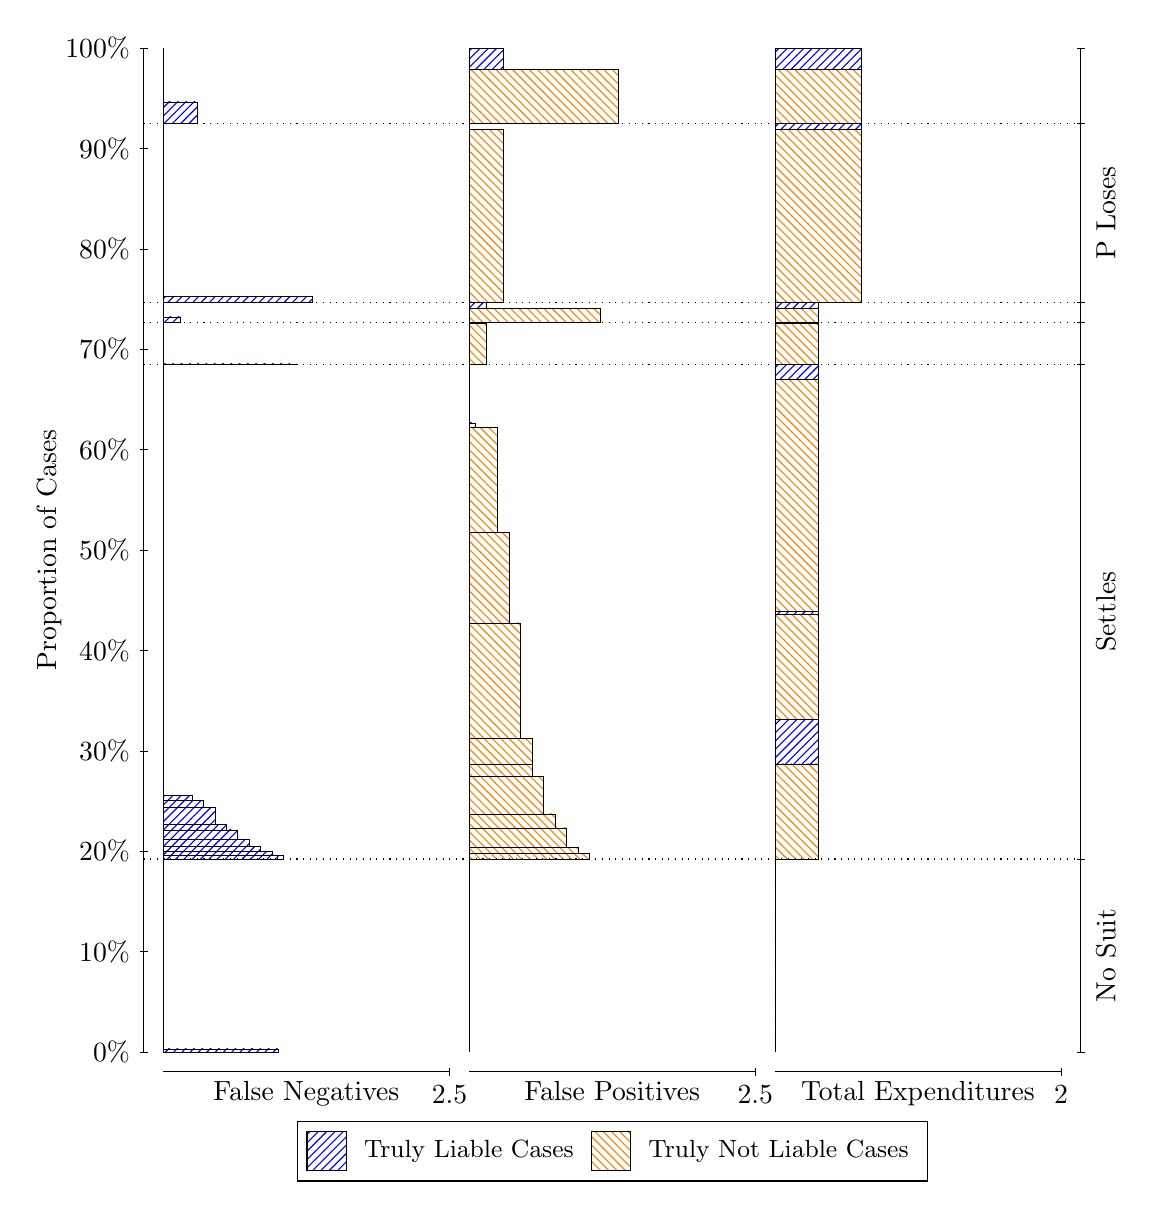
\begin{tikzpicture}
\draw[black, very thin] (1.5,1.75) -- (1.5,14.5);
\node[rotate=90, text=black, anchor=center] at (0.3, 8.125) {Proportion of Cases};
\draw[black, very thin] (1.45,1.75) -- (1.55,1.75);
\node[text=black, anchor=east] at (1.45, 1.75) {0\%};
\draw[black, very thin] (1.45,3.025) -- (1.55,3.025);
\node[text=black, anchor=east] at (1.45, 3.025) {10\%};
\draw[black, very thin] (1.45,4.3) -- (1.55,4.3);
\node[text=black, anchor=east] at (1.45, 4.3) {20\%};
\draw[black, very thin] (1.45,5.575) -- (1.55,5.575);
\node[text=black, anchor=east] at (1.45, 5.575) {30\%};
\draw[black, very thin] (1.45,6.85) -- (1.55,6.85);
\node[text=black, anchor=east] at (1.45, 6.85) {40\%};
\draw[black, very thin] (1.45,8.125) -- (1.55,8.125);
\node[text=black, anchor=east] at (1.45, 8.125) {50\%};
\draw[black, very thin] (1.45,9.4) -- (1.55,9.4);
\node[text=black, anchor=east] at (1.45, 9.4) {60\%};
\draw[black, very thin] (1.45,10.675) -- (1.55,10.675);
\node[text=black, anchor=east] at (1.45, 10.675) {70\%};
\draw[black, very thin] (1.45,11.95) -- (1.55,11.95);
\node[text=black, anchor=east] at (1.45, 11.95) {80\%};
\draw[black, very thin] (1.45,13.225) -- (1.55,13.225);
\node[text=black, anchor=east] at (1.45, 13.225) {90\%};
\draw[black, very thin] (1.45,14.5) -- (1.55,14.5);
\node[text=black, anchor=east] at (1.45, 14.5) {100\%};

\draw[black, very thin] (13.4,1.75) -- (13.4,14.5);
\draw[black, very thin] (13.35,1.75) -- (13.45,1.75);
\node[anchor=west] at (13.35, 1.75) {};
\draw[black, very thin] (13.35,4.2008) -- (13.45,4.2008);
\node[anchor=west] at (13.35, 4.2008) {};
\draw[black, very thin] (13.35,10.481) -- (13.45,10.481);
\node[anchor=west] at (13.35, 10.481) {};
\draw[black, very thin] (13.35,11.013) -- (13.45,11.013);
\node[anchor=west] at (13.35, 11.013) {};
\draw[black, very thin] (13.35,11.269) -- (13.45,11.269);
\node[anchor=west] at (13.35, 11.269) {};
\draw[black, very thin] (13.35,13.541) -- (13.45,13.541);
\node[anchor=west] at (13.35, 13.541) {};
\draw[black, very thin] (13.35,14.5) -- (13.45,14.5);
\node[anchor=west] at (13.35, 14.5) {};

\draw[black, very thin, pattern color=blue, pattern=north east lines] (1.75,1.75) rectangle (3.2033,1.7904);
\draw[black, very thin, pattern color=orange, pattern=north west lines] (1.75,1.7904) rectangle (1.75,4.2008);
\draw[black, very thin, pattern color=blue, pattern=north east lines] (1.75,4.2008) rectangle (3.276,4.2452);
\draw[black, very thin, pattern color=blue, pattern=north east lines] (1.75,4.2452) rectangle (3.1307,4.2954);
\draw[black, very thin, pattern color=blue, pattern=north east lines] (1.75,4.2954) rectangle (2.9853,4.3657);
\draw[black, very thin, pattern color=blue, pattern=north east lines] (1.75,4.3657) rectangle (2.84,4.4499);
\draw[black, very thin, pattern color=blue, pattern=north east lines] (1.75,4.4499) rectangle (2.6947,4.5695);
\draw[black, very thin, pattern color=blue, pattern=north east lines] (1.75,4.5695) rectangle (2.5493,4.6406);
\draw[black, very thin, pattern color=blue, pattern=north east lines] (1.75,4.6406) rectangle (2.404,4.8603);
\draw[black, very thin, pattern color=blue, pattern=north east lines] (1.75,4.8603) rectangle (2.2587,4.943);
\draw[black, very thin, pattern color=blue, pattern=north east lines] (1.75,4.943) rectangle (2.1133,5.0039);
\draw[black, very thin, pattern color=orange, pattern=north west lines] (1.75,5.0039) rectangle (1.75,10.481);
\draw[black, very thin, pattern color=blue, pattern=north east lines] (1.75,10.481) rectangle (3.4213,10.49);
\draw[black, very thin, pattern color=orange, pattern=north west lines] (1.75,10.49) rectangle (1.75,11.013);
\draw[black, very thin, pattern color=blue, pattern=north east lines] (1.75,11.013) rectangle (1.968,11.086);
\draw[black, very thin, pattern color=orange, pattern=north west lines] (1.75,11.086) rectangle (1.75,11.269);
\draw[black, very thin, pattern color=blue, pattern=north east lines] (1.75,11.269) rectangle (3.6393,11.345);
\draw[black, very thin, pattern color=orange, pattern=north west lines] (1.75,11.345) rectangle (1.75,13.541);
\draw[black, very thin, pattern color=blue, pattern=north east lines] (1.75,13.541) rectangle (2.186,13.815);
\draw[black, very thin, pattern color=orange, pattern=north west lines] (1.75,13.815) rectangle (1.75,14.5);
\draw[black, very thin, pattern color=orange, pattern=north west lines] (5.6333,1.75) rectangle (5.6333,4.1604);
\draw[black, very thin, pattern color=blue, pattern=north east lines] (5.6333,4.1604) rectangle (5.6333,4.2008);
\draw[black, very thin, pattern color=orange, pattern=north west lines] (5.6333,4.2008) rectangle (7.1593,4.2692);
\draw[black, very thin, pattern color=orange, pattern=north west lines] (5.6333,4.2692) rectangle (7.014,4.3474);
\draw[black, very thin, pattern color=orange, pattern=north west lines] (5.6333,4.3474) rectangle (6.8687,4.5947);
\draw[black, very thin, pattern color=orange, pattern=north west lines] (5.6333,4.5947) rectangle (6.7233,4.7739);
\draw[black, very thin, pattern color=orange, pattern=north west lines] (5.6333,4.7739) rectangle (6.578,5.2466);
\draw[black, very thin, pattern color=orange, pattern=north west lines] (5.6333,5.2466) rectangle (6.4327,5.4077);
\draw[black, very thin, pattern color=orange, pattern=north west lines] (5.6333,5.4077) rectangle (6.4327,5.7335);
\draw[black, very thin, pattern color=orange, pattern=north west lines] (5.6333,5.7335) rectangle (6.2873,7.1986);
\draw[black, very thin, pattern color=orange, pattern=north west lines] (5.6333,7.1986) rectangle (6.142,8.3524);
\draw[black, very thin, pattern color=orange, pattern=north west lines] (5.6333,8.3524) rectangle (5.9967,9.6776);
\draw[black, very thin, pattern color=blue, pattern=north east lines] (5.6333,9.6776) rectangle (5.706,9.7385);
\draw[black, very thin, pattern color=blue, pattern=north east lines] (5.6333,9.7385) rectangle (5.6333,10.481);
\draw[black, very thin, pattern color=orange, pattern=north west lines] (5.6333,10.481) rectangle (5.8513,11.004);
\draw[black, very thin, pattern color=blue, pattern=north east lines] (5.6333,11.004) rectangle (5.6333,11.013);
\draw[black, very thin, pattern color=orange, pattern=north west lines] (5.6333,11.013) rectangle (7.3047,11.197);
\draw[black, very thin, pattern color=blue, pattern=north east lines] (5.6333,11.197) rectangle (5.8513,11.269);
\draw[black, very thin, pattern color=orange, pattern=north west lines] (5.6333,11.269) rectangle (6.0693,13.465);
\draw[black, very thin, pattern color=blue, pattern=north east lines] (5.6333,13.465) rectangle (5.6333,13.541);
\draw[black, very thin, pattern color=orange, pattern=north west lines] (5.6333,13.541) rectangle (7.5227,14.226);
\draw[black, very thin, pattern color=blue, pattern=north east lines] (5.6333,14.226) rectangle (6.0693,14.5);
\draw[black, very thin, pattern color=orange, pattern=north west lines] (9.5167,1.75) rectangle (9.5167,4.1604);
\draw[black, very thin, pattern color=blue, pattern=north east lines] (9.5167,4.1604) rectangle (9.5167,4.2008);
\draw[black, very thin, pattern color=orange, pattern=north west lines] (9.5167,4.2008) rectangle (10.062,5.4077);
\draw[black, very thin, pattern color=blue, pattern=north east lines] (9.5167,5.4077) rectangle (10.062,5.9786);
\draw[black, very thin, pattern color=orange, pattern=north west lines] (9.5167,5.9786) rectangle (10.062,7.3038);
\draw[black, very thin, pattern color=blue, pattern=north east lines] (9.5167,7.3038) rectangle (10.062,7.3482);
\draw[black, very thin, pattern color=orange, pattern=north west lines] (9.5167,7.3482) rectangle (10.062,10.293);
\draw[black, very thin, pattern color=blue, pattern=north east lines] (9.5167,10.293) rectangle (10.062,10.481);
\draw[black, very thin, pattern color=orange, pattern=north west lines] (9.5167,10.481) rectangle (10.062,11.004);
\draw[black, very thin, pattern color=blue, pattern=north east lines] (9.5167,11.004) rectangle (10.062,11.013);
\draw[black, very thin, pattern color=orange, pattern=north west lines] (9.5167,11.013) rectangle (10.062,11.197);
\draw[black, very thin, pattern color=blue, pattern=north east lines] (9.5167,11.197) rectangle (10.062,11.269);
\draw[black, very thin, pattern color=orange, pattern=north west lines] (9.5167,11.269) rectangle (10.607,13.465);
\draw[black, very thin, pattern color=blue, pattern=north east lines] (9.5167,13.465) rectangle (10.607,13.541);
\draw[black, very thin, pattern color=orange, pattern=north west lines] (9.5167,13.541) rectangle (10.607,14.226);
\draw[black, very thin, pattern color=blue, pattern=north east lines] (9.5167,14.226) rectangle (10.607,14.5);
\draw[black, dotted] (1.5,4.2008) -- (13.4,4.2008);
\draw[black, dotted] (1.5,10.481) -- (13.4,10.481);
\draw[black, dotted] (1.5,11.013) -- (13.4,11.013);
\draw[black, dotted] (1.5,11.269) -- (13.4,11.269);
\draw[black, dotted] (1.5,13.541) -- (13.4,13.541);
\draw[black, very thin] (1.75,1.5) -- (5.3833,1.5);
\node[text=black, anchor=north] at (3.5667, 1.5) {False Negatives};
\draw[black, very thin] (5.3833,1.45) -- (5.3833,1.55);
\node[text=black, anchor=north] at (5.3833, 1.45) {2.5};

\draw[black, very thin] (5.6333,1.5) -- (9.2667,1.5);
\node[text=black, anchor=north] at (7.45, 1.5) {False Positives};
\draw[black, very thin] (9.2667,1.45) -- (9.2667,1.55);
\node[text=black, anchor=north] at (9.2667, 1.45) {2.5};

\draw[black, very thin] (9.5167,1.5) -- (13.15,1.5);
\node[text=black, anchor=north] at (11.333, 1.5) {Total Expenditures};
\draw[black, very thin] (13.15,1.45) -- (13.15,1.55);
\node[text=black, anchor=north] at (13.15, 1.45) {2};

\node[text=black, centered, rotate=90] at (13.72, 2.9754) {No Suit};
\node[text=black, centered, rotate=90] at (13.72, 7.3407) {Settles};


\node[text=black, centered, rotate=90] at (13.72, 12.405) {P Loses};


\draw (7.449999999999999,1.5) node[draw=none] (baseCoordinate) {};
\begin{scope}[align=center]
        \matrix[scale=0.5, draw=black, below=0.5cm of baseCoordinate, nodes={draw}, column sep=0.1cm]{
            \node[rectangle, draw, minimum width=0.5cm, minimum height=0.5cm, pattern color=blue, pattern=north east lines] {}; &
            \node[draw=none, font=\small, text=black] (B) {Truly Liable Cases}; &
            \node[rectangle, draw, minimum width=0.5cm, minimum height=0.5cm, pattern color=orange, pattern=north west lines] {}; &
            \node[draw=none, font=\small, text=black] (B) {Truly Not Liable Cases}; \\
            };
\end{scope}

\end{tikzpicture}
\end{document}